\documentclass[a4paper, twoside, english]{article}

\usepackage{amsmath}
\usepackage{amsfonts}
\usepackage{ihci}
\usepackage{graphicx}
\usepackage{subfig}
\usepackage{listings}
\usepackage{color}

% Unicode workaround for lstlistings
\lstset{literate=
	{á}{{\'a}}1 {é}{{\'e}}1 {í}{{\'i}}1 {ó}{{\'o}}1 {ú}{{\'u}}1
	{Á}{{\'A}}1 {É}{{\'E}}1 {Í}{{\'I}}1 {Ó}{{\'O}}1 {Ú}{{\'U}}1
	{à}{{\`a}}1 {è}{{\`e}}1 {ì}{{\`i}}1 {ò}{{\`o}}1 {ù}{{\`u}}1
	{À}{{\`A}}1 {È}{{\'E}}1 {Ì}{{\`I}}1 {Ò}{{\`O}}1 {Ù}{{\`U}}1
	{ä}{{\"a}}1 {ë}{{\"e}}1 {ï}{{\"i}}1 {ö}{{\"o}}1 {ü}{{\"u}}1
	{Ä}{{\"A}}1 {Ë}{{\"E}}1 {Ï}{{\"I}}1 {Ö}{{\"O}}1 {Ü}{{\"U}}1
	{â}{{\^a}}1 {ê}{{\^e}}1 {î}{{\^i}}1 {ô}{{\^o}}1 {û}{{\^u}}1
	{Â}{{\^A}}1 {Ê}{{\^E}}1 {Î}{{\^I}}1 {Ô}{{\^O}}1 {Û}{{\^U}}1
	{œ}{{\oe}}1 {Œ}{{\OE}}1 {æ}{{\ae}}1 {Æ}{{\AE}}1 {ß}{{\ss}}1
	{ű}{{\H{u}}}1 {Ű}{{\H{U}}}1 {ő}{{\H{o}}}1 {Ő}{{\H{O}}}1
	{ç}{{\c c}}1 {Ç}{{\c C}}1 {ø}{{\o}}1 {å}{{\r a}}1 {Å}{{\r A}}1
	{€}{{\euro}}1 {£}{{\pounds}}1 {«}{{\guillemotleft}}1
	{»}{{\guillemotright}}1 {ñ}{{\~n}}1 {Ñ}{{\~N}}1 {¿}{{?`}}1
}

% Define Synatx highlighting for Python
\definecolor{maroon}{cmyk}{0, 0.87, 0.68, 0.32}
\definecolor{halfgray}{gray}{0.55}
\definecolor{ipython_frame}{RGB}{207, 207, 207}
\definecolor{ipython_bg}{RGB}{247, 247, 247}
\definecolor{ipython_red}{RGB}{186, 33, 33}
\definecolor{ipython_green}{RGB}{0, 128, 0}
\definecolor{ipython_cyan}{RGB}{64, 128, 128}
\definecolor{ipython_purple}{RGB}{170, 34, 255}

\lstdefinelanguage{iPython}{
	morekeywords=[1]{access,and,break,class,continue,def,del,elif,else,except,exec,finally,for,from,global,if,import,in,is,lambda,not,or,pass,print,raise,return,try,while},%
	%
	% Built-ins
	morekeywords=[2]{abs,all,any,basestring,bin,bool,bytearray,callable,chr,classmethod,cmp,compile,complex,delattr,dict,dir,divmod,enumerate,eval,execfile,file,filter,float,format,frozenset,getattr,globals,hasattr,hash,help,hex,id,input,int,isinstance,issubclass,iter,len,list,locals,long,map,max,memoryview,min,next,object,oct,open,ord,pow,property,range,raw_input,reduce,reload,repr,reversed,round,set,setattr,slice,sorted,staticmethod,str,sum,super,tuple,type,unichr,unicode,vars,xrange,zip,apply,buffer,coerce,intern},%
	%
	sensitive=true,%
	morecomment=[l]\#,%
	morestring=[b]',%
	morestring=[b]",%
	%
	morestring=[s]{'''}{'''},% used for documentation text (mulitiline strings)
	morestring=[s]{"""}{"""},% added by Philipp Matthias Hahn
	%
	morestring=[s]{r'}{'},% `raw' strings
	morestring=[s]{r"}{"},%
	morestring=[s]{r'''}{'''},%
	morestring=[s]{r"""}{"""},%
	morestring=[s]{u'}{'},% unicode strings
	morestring=[s]{u"}{"},%
	morestring=[s]{u'''}{'''},%
	morestring=[s]{u"""}{"""},%
	morestring=[s]{f'}{'},% format strings
	morestring=[s]{f"}{"},%
	morestring=[s]{f'''}{'''},%
	morestring=[s]{f"""}{"""},%
	%
	identifierstyle=\color{black}\ttfamily,
	commentstyle=\color{ipython_cyan}\ttfamily,
	stringstyle=\color{ipython_red}\ttfamily,
	keepspaces=true,
	showspaces=false,
	showstringspaces=false,
	%
	rulecolor=\color{ipython_frame},
	frame=single,
	frameround={t}{t}{t}{t},
	framexleftmargin=7mm,
	numbers=left,
	numberstyle=\tiny\color{halfgray},
	%
	%
	backgroundcolor=\color{ipython_bg},
	extendedchars=true,
	basicstyle={\footnotesize\ttfamily},
	keywordstyle=[1]{\color{ipython_green}\ttfamily},
	keywordstyle=[2]{\color{ipython_purple}\ttfamily},
}

\graphicspath{{./../figures/}}

\title{Machine Learning Project\\Task 2 Report}  
\author{Albert Garaev,\\ Ksenia Novikova,\\ Mukhammadsodik Khabibulloev }    
\date{04.01.2022}                              

\begin{document}

\maketitle


\section{Data Pre-processing}

We download the dataset wich contains  wine reviews and other information about wine as a pandas DataFrame. The Figure\ref{fig:data} shows the view of our data.\\
~\\
\begin{figure}[h!]
	\centerline{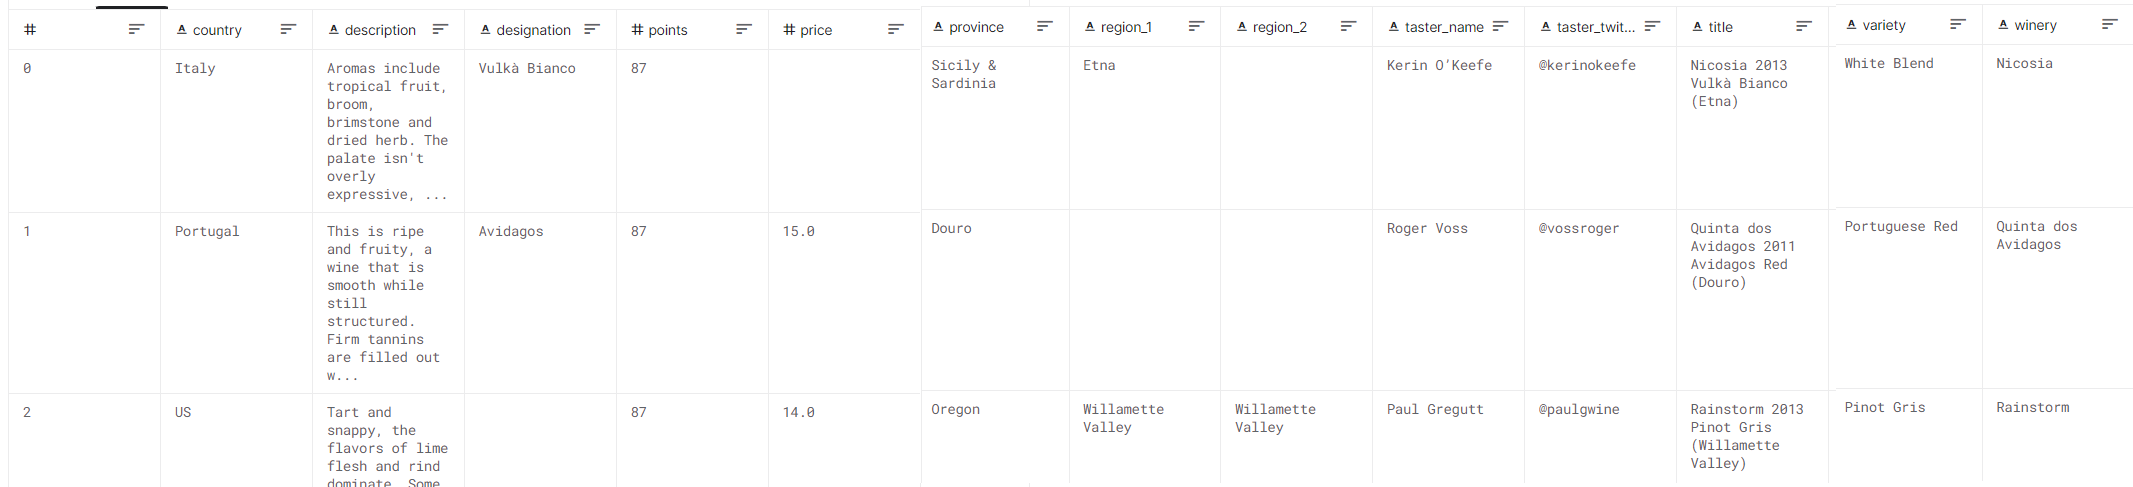
\includegraphics[width=\textwidth]{data.png}}
	\caption[data]{View of the dataset}
	\label{fig:data}
\end{figure}\\


We need to extract the wine's years from the title column and add them as a new column to our data. We write a function below.\\
\begin{lstlisting}[language=iPython]
Year = []
for value in wines['title']:
	result = re.search(r'19\d{2}|20\d{2}', value)
	if result:
		Year.append(float(result.group()))
	else: Year.append(np.nan)

wines['year'] = Year
\end{lstlisting}


~\\
We can plot a histogram for each columns. We group the numerecal into bins as usual, for ither types of data we count each unique value and order them on the x-axis by descending count. The Figure \ref{fig:hist1} shows histogram for numerical data.\\


\begin{figure}[h!]
	\centerline{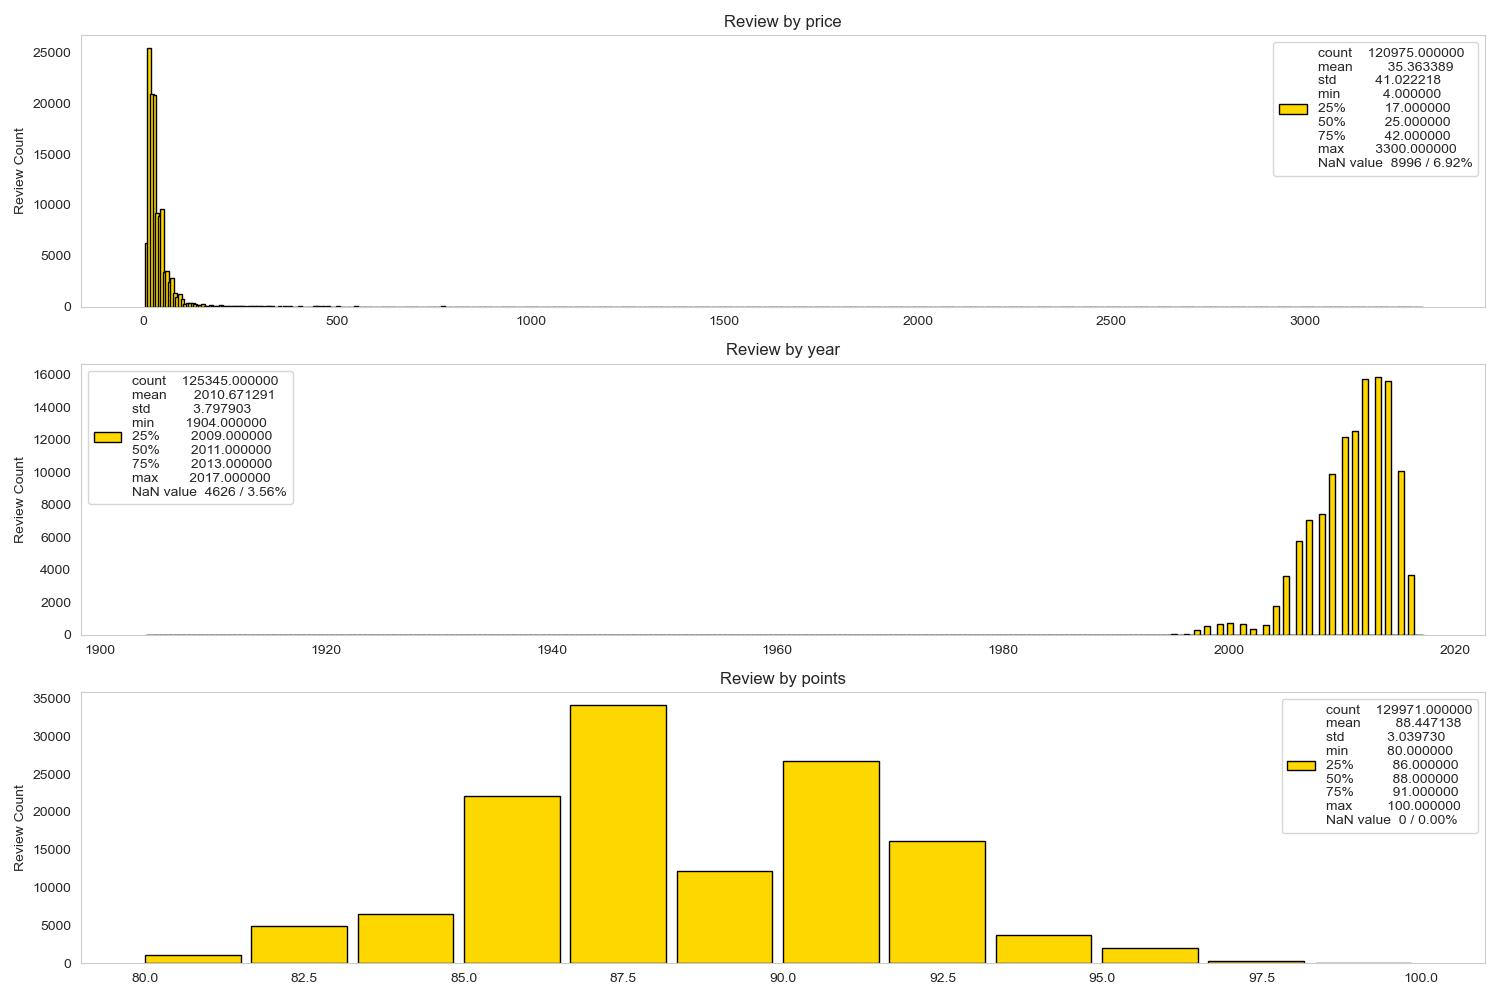
\includegraphics[width=0.75\textwidth]{hist1.png}}
	\caption[hist]{Histograms for numerical data}
	\label{fig:hist1}
\end{figure}
\newpage


The Figure\ref{fig:hist2} shows histogram for other data.\\
 \begin{figure}[h!]
	\centerline
	{
		\subfloat[]{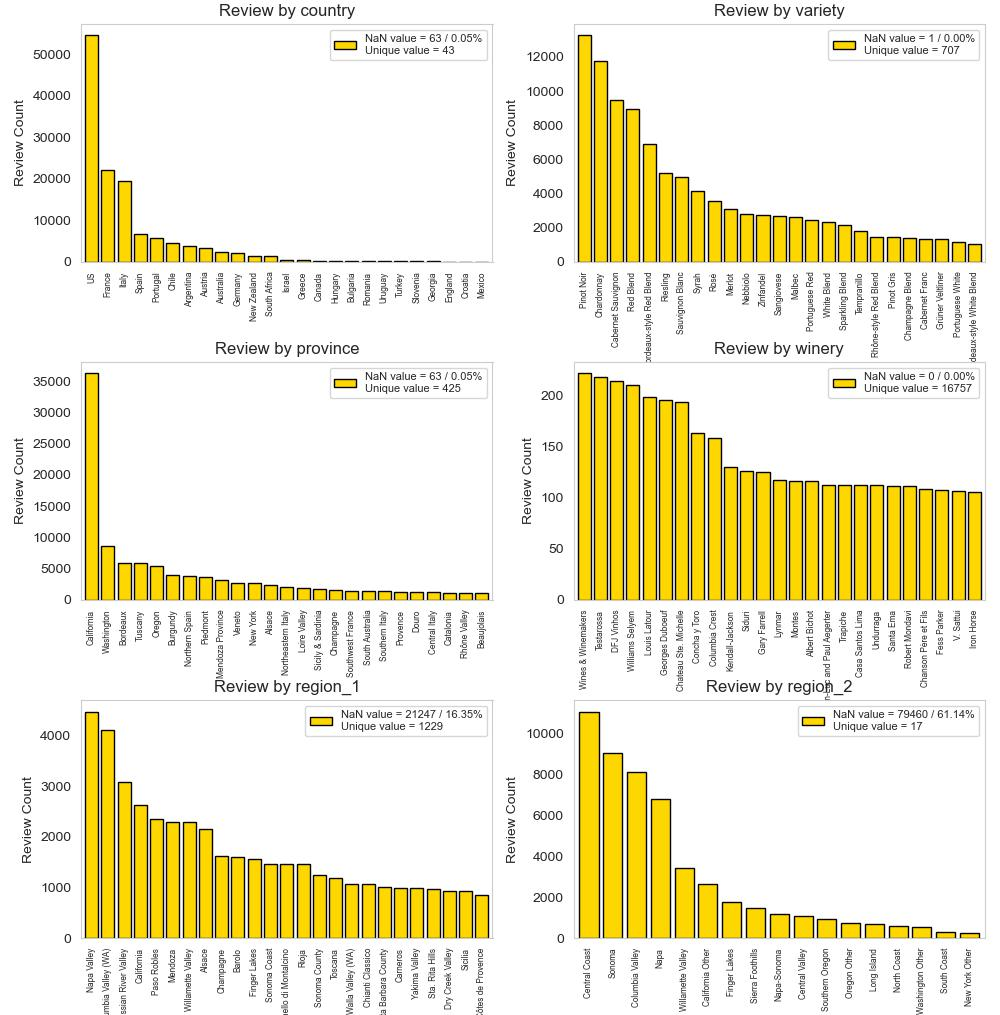
\includegraphics[width=0.55\textwidth]{hist2.png}}
		\qquad
		\subfloat[]{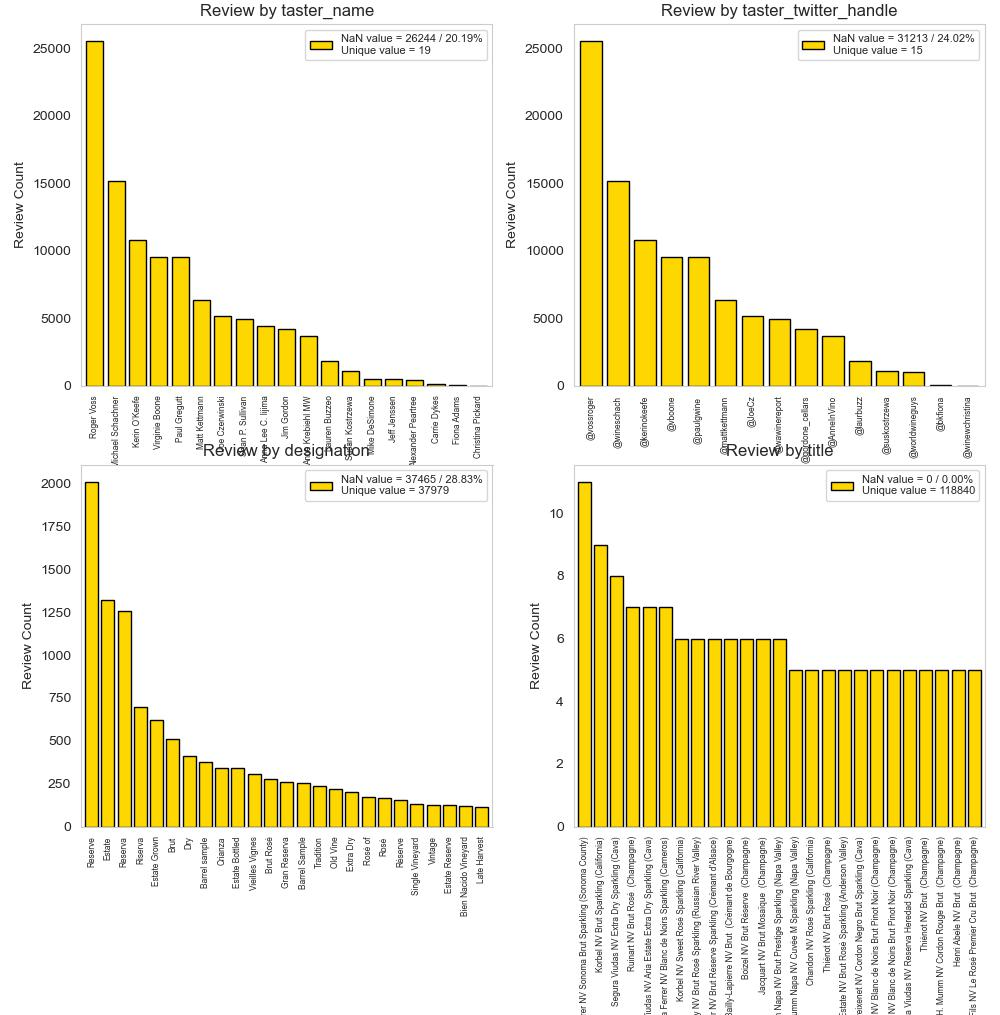
\includegraphics[width=0.55\textwidth]{hist3.png}}
	}
	\caption[hist]{Histograms for other data}
	\label{fig:hist2}
\end{figure}


\newpage

We use $pandas.isna(obj)$, which detect missing values for an array-like object, to show how many of the values are
missing for each column. $pandas.DataFrame.describe()$ generates descriptive statistics  for numeric data such as count, mean, std, min, max as well as lower (default is 25), 50 and upper (default 75) percentiles, the 50 percentile is the same as the median ~\cite{Pandas}\\
~\\
We need to transform our data into real numbers. Also we need to  handle with missing(NaN) values.\\
~\\
We implement $nullscan(df)$, where we perofrm the nullscan for a dataframe. The $pandas.isna(obj)$ returns boolean value. Dataframe (the size of the original dataframe) contain value True in null-cells and value False in the other cells. After we interpret True as 1 and False  as 0. We can see after using $nullscan(df)$ that the dataset contains missing values and we need to handle them.\\
~\\
\begin{lstlisting}[language=iPython]
def nullsearch(wines_check):
	wines_nulls = wines_check.isna()
	nulls_per_col = wines_nulls.sum(axis=0)
	nulls_per_col /= len(wines_check.index)
	
	with plt.style.context('dark_background'):
			figure_5, (ax1, ax2) = plt.subplots(nrows=2, ncols=1, 
			sharex=True, figsize=(6, 8))
		vir = matplotlib.cm.get_cmap('viridis')
		colormap = matplotlib.colors.ListedColormap([vir(0), 'white'])
		sns.heatmap(wines_check.isnull(), cmap=colormap, cbar=False, 
		yticklabels=False, ax=ax1)
		
		nulls_per_col.plot(kind='bar', color='white', x=nulls_per_col.values,
		y=nulls_per_col.index, ax=ax2, width=1, linewidth=1,
		edgecolor='black', align='edge', label='NaN value rate')
		
		ax2.set_ylim((0, 1))
		# centered labels
		labels = wines_check.columns
		ticks = np.arange(0.5, len(labels))
		ax2.xaxis.set(ticks=ticks, ticklabels=labels)
		
		ax2.spines['top'].set_color('black')
		ax2.spines['right'].set_color('black')
		
		#very small amounts of NaN values per column
		na_ticks = ticks[(nulls_per_col > 0) & (nulls_per_col < 0.05)]
		if (len(na_ticks) > 0):
		ax2.plot(na_ticks, [0, ] * len(na_ticks), 's', c='white', markersize=10,
		label='Very few missing values')
		
		figure_5.suptitle('NaN values evaluation', fontsize=30, y=1.05)
		ax2.legend()
		figure_5.tight_layout()
		plt.show()

nullsearch(wines)
\end{lstlisting}
\newpage
The Figure \ref{fig:null1} shows the rate of null-values in each column.\\
\begin{figure}[h!]
	\centerline{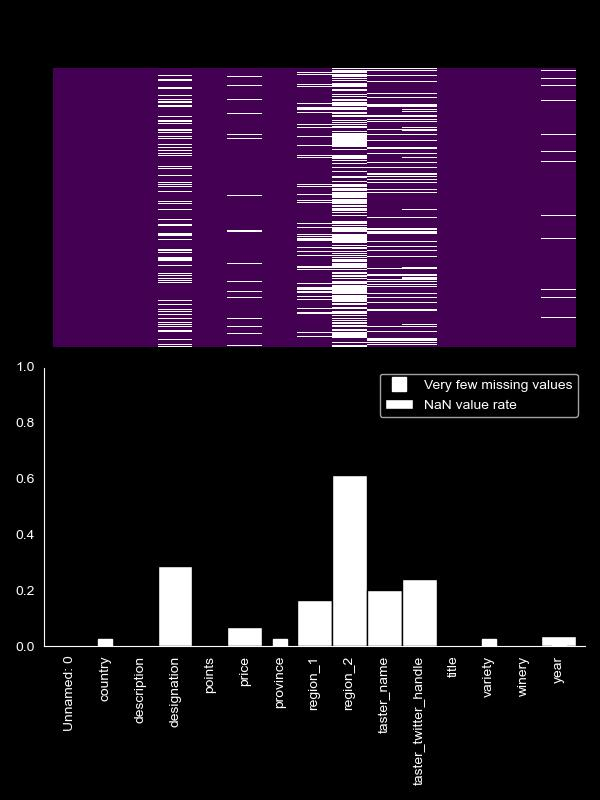
\includegraphics[width=0.40\textwidth]{null1.png}}
	\caption[null]{Amount of NaN values in each column}
	\label{fig:null1}
\end{figure}


There are many methods to handle Null Values. We choose method of droping columns, wich contains a specified amount of null-values, if the number of missing values is very high and the column isn't too relevant. \\
The Figure \ref{fig:null2} shows the rate of null-values after dropping some columns.\\
\begin{figure}[h!]
	\centerline{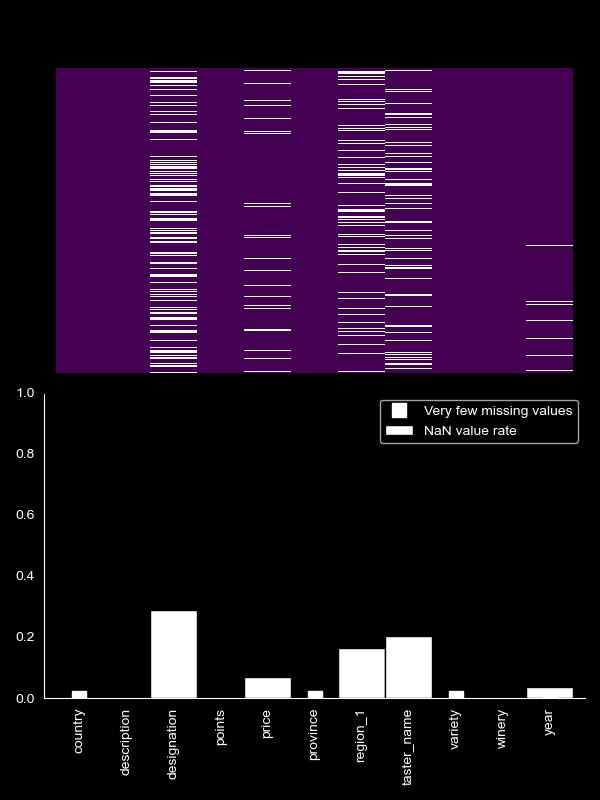
\includegraphics[width=0.40\textwidth]{null2.png}}
	\caption[null]{Amount of NaN values in each column after columns dropping}
	\label{fig:null2}
\end{figure}
\newpage
After that we change NaN-values to the "Unknown". The Figure \ref{fig:null3} shows the columns after changing.\\
\begin{figure}[h!]
	\centerline{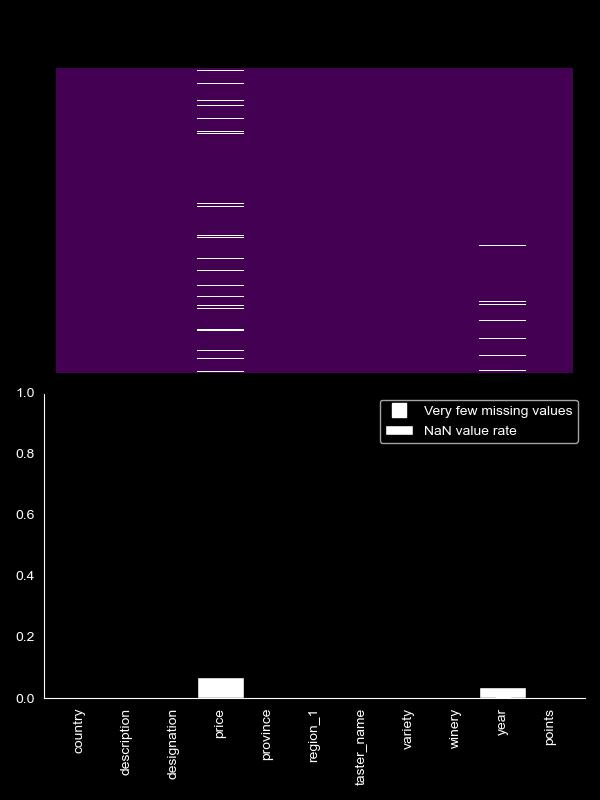
\includegraphics[width=0.45\textwidth]{null3.png}}
	\caption[null]{Columns after changing to the "Unknown"-values}
	\label{fig:null3}
\end{figure}

At last, we predict  null-values at the columns "price" and "year" using KNN method. The Figure \ref{fig:null45} shows the results for columns "Price" and "Year".\\
 \begin{figure}[h!]
	\centerline
	{
		\subfloat[]{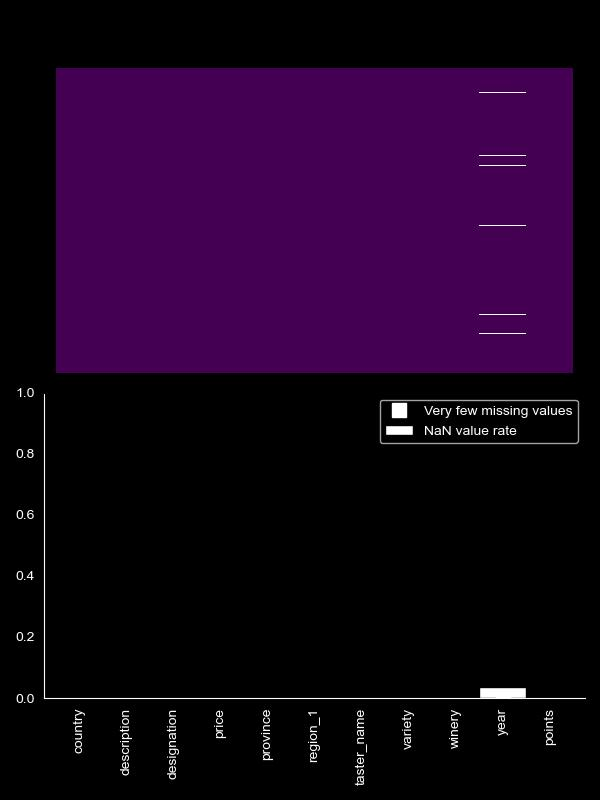
\includegraphics[width=0.40\textwidth]{null4.png}}
		\qquad
		\subfloat[]{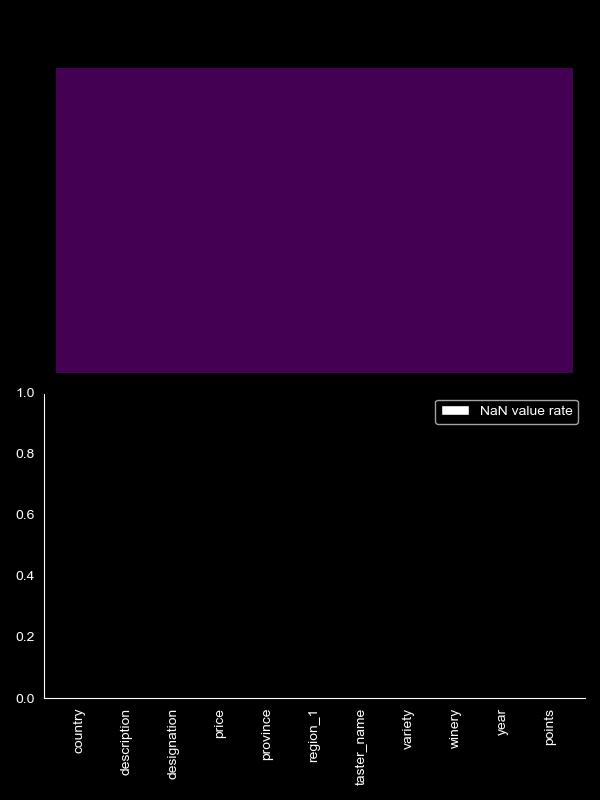
\includegraphics[width=0.40\textwidth]{null5.png}}
	}
	\caption[null]{Predicted values for columns a)"Price", b)"Year"}
	\label{fig:null45}
\end{figure}
\newpage
After we can transofm the categorical data into numbers. We use $LabelEncoder$ for data tranformation and create dictionary with our transformed into numbers categorical data. This method is easy to impliment. After we transform text columns using Word2Vec algorithm. This algorithm was used due to ease of use, open source code and speed. We download a pre-trained word2vec model by google $GoogleNews-vectors-negative300.bin$. After that we can transform the dataset row by row, checking is data categorical or text and using functions wich was described above.\\

Pre-processing our data. Type of wine is a text data type. In this case, the Word2Vec function is used for processing. At first, the vector is initialized to zero. After that, words are searched for in the model dictionary. If the search is successful, the vector becomes numeric, otherwise (the word was not found in the dictionary) the vector remains zero. The best solution might be to increase the dictionary so that no exceptions are thrown and all text variables (in our case the type of wine) are converted to numeric vectors.\\

Outliers have a huge impact on data quality. We should definitely detect outliers for several reasons. Outliers distort the overall picture and thus reduce accuracy. Probably the best known way to detect outliers is using a z-score. We use $scipy.stats.zscore()$ for this task.\\


\section{Regression}
We implement a class $RidgeRegression$.
\begin{lstlisting}[language=iPython]
class RidgeRegression:
	def init(self, C):
		self.C = C
		self.w = None
	
	def fit(self, X, y):
		self.w = np.linalg.inv(X.T @ X + (1 / self.C) * np.eye(X.shape[1])) @ (X.T @ y)
	
	def predict(self, X):
		return np.dot(X, self.w)
	
	def calc_metrics(self, X_train, y_train, X_test, y_test):
		self.fit(X_train, y_train)
		train_error = self.calc_error(X_train, y_train)
		validation_error = self.calc_error(X_test, y_test)
		return train_error, validation_error
\end{lstlisting}
We use Principal component analysis (PCA). This is one of the main ways to reduce the dimension of data, losing the least amount of information. The method reduces the linear dimension by using singular value decomposition to project it into a lower-dimensional space. In this case, for each function before SVD is applied, the input is centered but not scaled.\\
Thus we can see in Figure\ref{fig:scatter} scatter plot that shows the projected value of the column and line wich is result of of ridge regression.\\
%3 рисунка
 \begin{figure}[h!]
 \centerline
{
	\subfloat[]{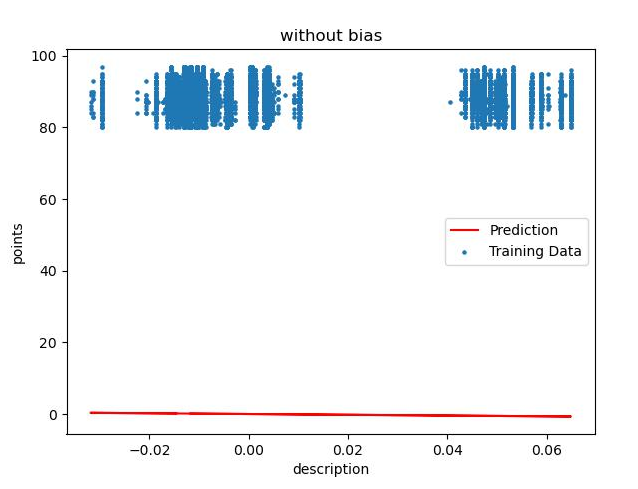
\includegraphics[width=0.35\textwidth]{scatter_desc.png}}
	\qquad
	\subfloat[]{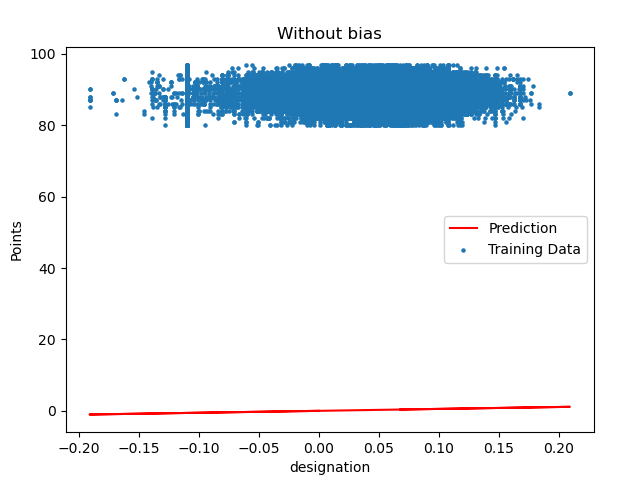
\includegraphics[width=0.35\textwidth]{scatter_desi.png}}
	\qquad
	\subfloat[]{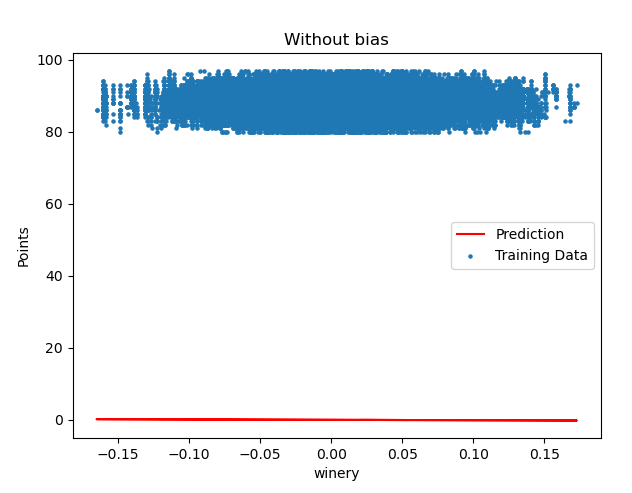
\includegraphics[width=0.35\textwidth]{scatter_win.png}}
}
\caption[scatter]{Scatter plot for ridge regression without bias}
\label{fig:scatter}
\end{figure}


\newpage
We implement a new class $RidgeRegressionBias$ that uses the unchanged class $RidgeRegression$:\\
\begin{lstlisting}[language=iPython]
class RidgeRegressionBias(RidgeRegression):
	def fit(self, X, y):
		X = np.hstack((np.ones((X.shape[0], 1)), X))
		self.w = np.linalg.inv(X.T @ X + (1 / self.C) * np.eye(X.shape[1])) @ (X.T @ y)
	
	def calc_error(self, X, y):
		X = np.c_[np.ones(X.shape[0]), X]
		predictions = self.predict(X)
		mse = mean_squared_error(y, predictions)
		return mse
\end{lstlisting}
Bias is the ability of the algorithm model to adjust to the target dependence.\\
Thus we can see in Figure \ref{fig:scatter_b} scatter plot that shows the projected value of the column and line wich is result of ridge regression with bias.\\
%3 рисунка
 \begin{figure}[h!]
	\centerline
	{
		\subfloat[]{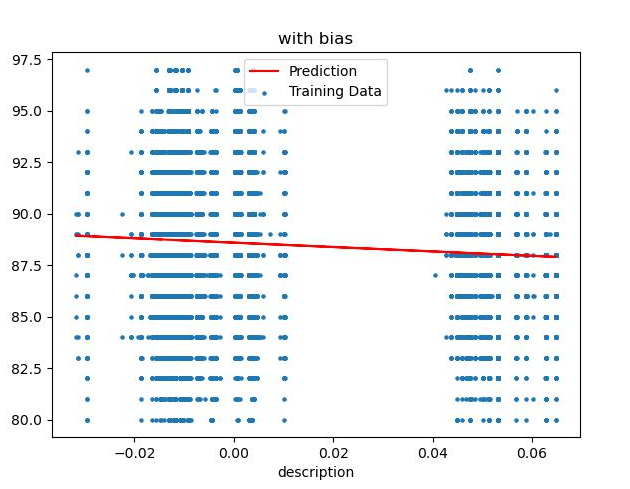
\includegraphics[width=0.35\textwidth]{scatter_b_desc.png}}
		\qquad
		\subfloat[]{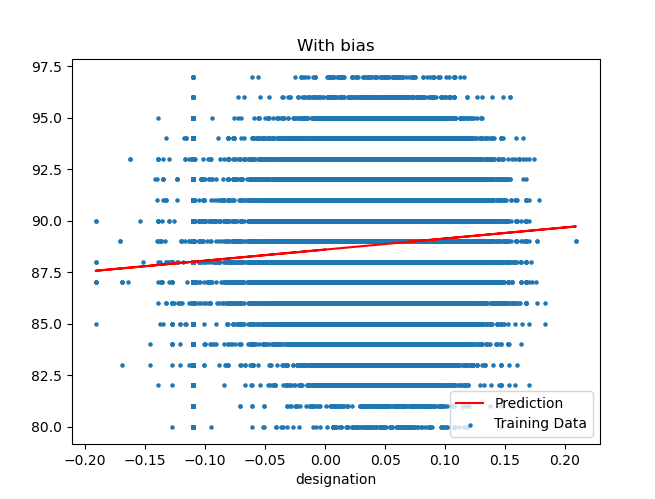
\includegraphics[width=0.35\textwidth]{scatter_b_desi.png}}
		\qquad
		\subfloat[]{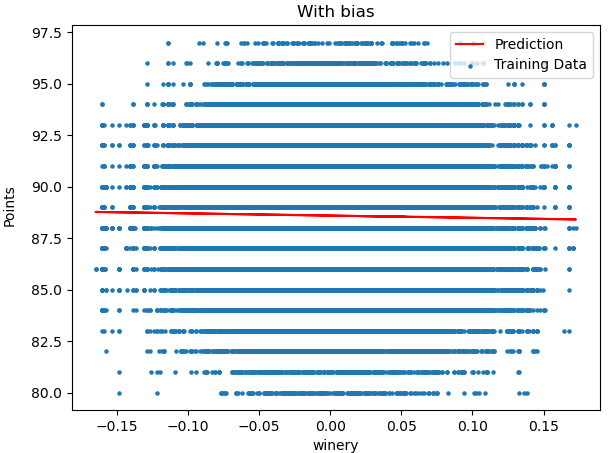
\includegraphics[width=0.35\textwidth]{scatter_b_win.png}}
	}
	\caption[scatter]{Scatter plot for ridge regression with bias}
	\label{fig:scatter_b}
\end{figure}


%MSE
We can now estimate the performance of our regressor using a fivefold cross validation and root mean square error (MSE) as a measure of performance. We implement $mean\_squared\_error()$ wich calculates mean squared error regression loss. We can see results in Table \ref{table:1}
\begin{center}
	\begin{table}[h!]
		\centering
		\begin{tabular}{||c c c c c c||} 
			\hline
			Type & K1 & K2 & K3 & K4 & K5 \\ [0.5ex] 
			\hline\hline
			Train errors in each Fold & 5.53 & 5.49 & 5.63 & 5.49 & 5.60 \\ 
			\hline
			Validation errors in each Fold & 5.64 & 5.79 & 5.23 & 5.79 & 5.36 \\ [1ex] 
			\hline
		\end{tabular}
		\caption{Values of mean square error (MSE)}
		\label{table:1}
	\end{table}
\end{center}

  
%Scaler
As we know each component $w_j$ of the weight vector is forced to be small in magnitude by the regularization term in ridge regression. The corresponding input feature $x_j$ can never contribute much to the final prediction, if the varies only slightly compared to the other features, although this may be important. In contrast, the corresponding feature's effect on the final prediction will be disproportionately large, if it takes values in a rather big interval. We can standardize features by removing the mean and scaling to unit variance to solve this problem. We use class sklearn $StandardScaler()$ to implement standardization. \\
\newpage

After that we compute mean squared error (MSE) again. We can see new results in Table \ref{table:2}
\begin{center}
	\begin{table}[h!]
		\centering
		\begin{tabular}{||c c c c c c||} 
			\hline
			Type & K1 & K2 & K3 & K4 & K5 \\ [0.5ex] 
			\hline\hline
			Train errors in each Fold & 5.42 & 5.38 & 5.52 & 5.39 & 5.48 \\ 
			\hline
			Validation errors in each Fold & 5.53 & 5.66 & 5.14 & 5.64 & 5.31 \\ [1ex] 
			\hline
		\end{tabular}
		\caption{Values of mean square error (MSE) using StandartScaler}
		\label{table:2}
	\end{table}
\end{center}

As wee can see value of MSE is smaller than before. So we can assume that in our case standardization helps us to recieve better results.

%Forward-Stepwise Selection
The essence of the Forward-Stepwise Selection is as follows: We start with a model that does not contain variables (called a null model).
Then we start adding the most significant variables one by one. Until the specified stopping rule is reached or until all the variables in question are included in the model. In our case, the stopping rule will be the inclusion of 3 variables in the model, since we found that this is enough to achieve an adequate estimate of the model.\\
 
 %Task 2g
We have a simple dataset which consists of scalar inputs and regression targets. We can see the plot of the dataset in Figure \ref{fig:task2g}. We can assume looking at the plot that this data was generated using standard normal distribution or t-distribution.

\begin{figure}[h!]
	\centerline{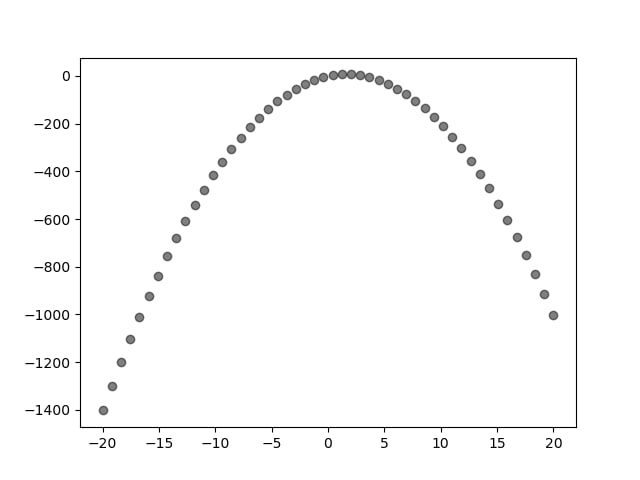
\includegraphics[width=0.55\textwidth]{task2g.png}}
	\caption[task2g]{Plot of the dataset }
	\label{fig:task2g}
\end{figure}
We apply our implementation of ridge regression on this data. The Figure \ref{fig:task2g_pr} the resulting line in the same plot as the data.\\
\begin{figure}[h!]
	\centerline{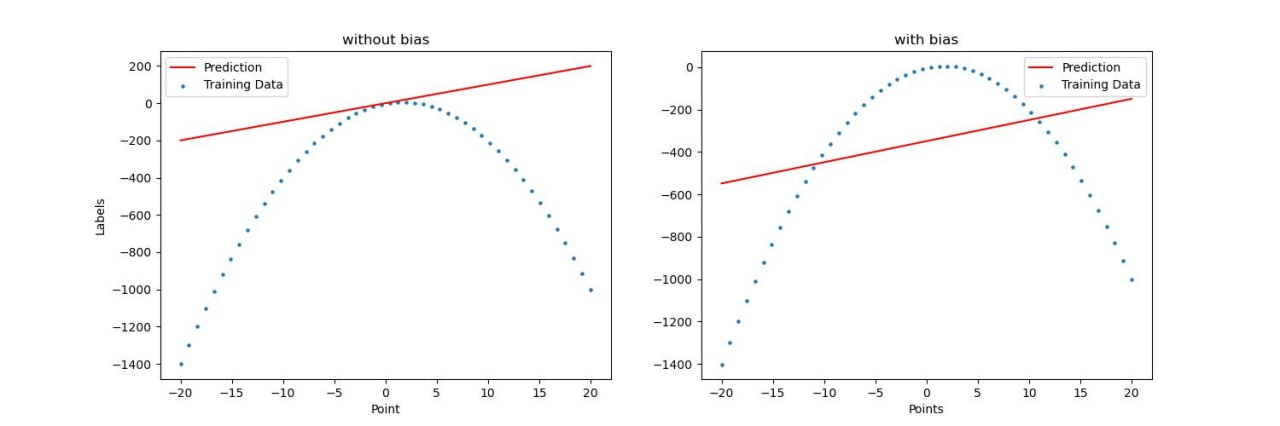
\includegraphics[width=0.85\textwidth]{task2g_pr.png}}
	\caption[task2g]{Plot of the dataset with resulting line}
	\label{fig:task2g_pr}
\end{figure}
\newpage

Ridge regression does not really work well in the case when the relation between input and target variables is not linear for a dataset. In this case the value of MSE is large (train error = 152084.58644527048 and test error = 103133.98900313386) and model can not be called adequate.\\
We need to find suitable $\phi$ in formula:
$f(x)=w^T\phi(x)+b=\sum\limits_{j=1}^d w_j \phi(x)_j+b $
~\\
~\\
We can see at the plot in Figure \ref{fig:task2g} that our data looks like parabola. We know the equation for this function: $y=ax^2+bx+c$, we also know the values of points. In this case, we constracted the system of equations and find approximate values $a\approx-3,\ b\approx10\ and\ c\approx-2$. After this expression $\phi$ becomes $\phi(x)=-3x^2+10x-2$.\\
Thus $f(x)=w^T(-3x^2+10x-2)+b=\sum\limits_{j=1}^d w_j (-3x_j^2+10x_j-2)+b $
~\\
~\\
Now the MSE close to zero: train error = 2.576008724130151e-07 and test error = 1.225935120189919e-07. The Figure \ref{fig:task2g_pr2} shows the plot with pridictions line.
\begin{figure}[h!]
	\centerline{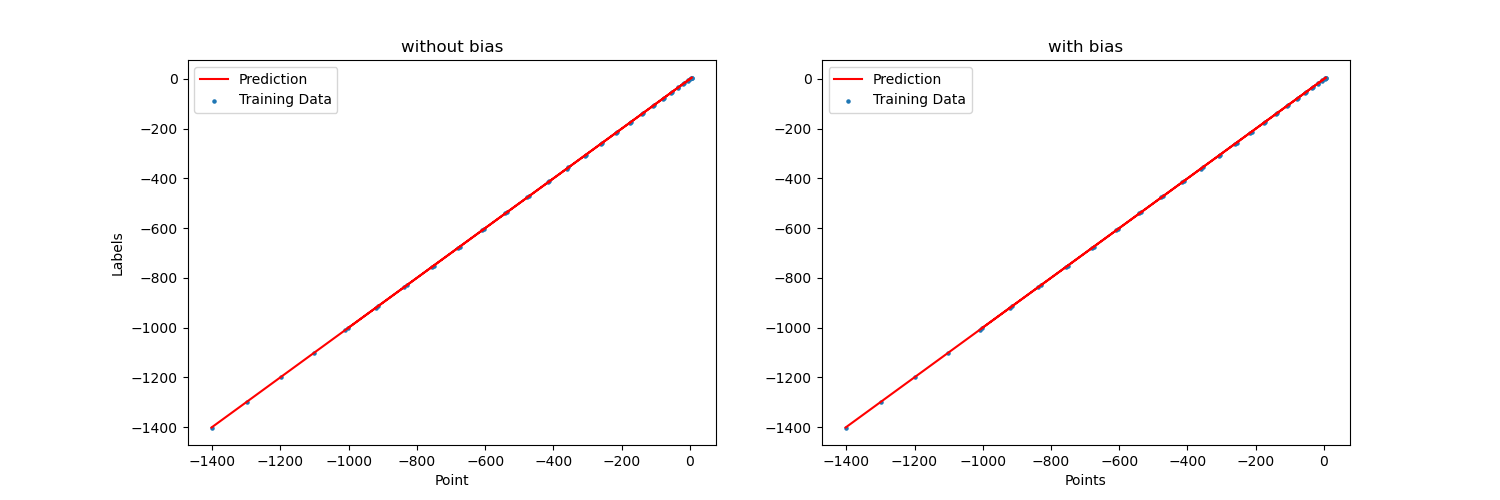
\includegraphics[width=0.85\textwidth]{task2g_pr2.png}}
	\caption[task2g]{Plot of the dataset with resulting line}
	\label{fig:task2g_pr2}
\end{figure}


\bibliographystyle{plain}
\bibliography{bibliography.bib}
\end{document}